\documentclass[tikz,border=12pt]{standalone}
\usepackage[T1]{fontenc}
\usepackage{mathpazo}
\usepackage{amsmath,amssymb}
\usetikzlibrary{arrows.meta, positioning, calc, fit, decorations.pathreplacing}

\definecolor{stblue}{HTML}{7B97AD}
\definecolor{rwgold}{HTML}{B8995E}
\definecolor{sage}{HTML}{7A9A7E}
\definecolor{dkbrown}{HTML}{3D3530}
\definecolor{wmgray}{HTML}{7B7067}
\definecolor{cream}{HTML}{F9F6F0}
\definecolor{border}{HTML}{D4C9B8}
\definecolor{terracotta}{HTML}{C47A6A}
\definecolor{lavender}{HTML}{907EA0}
\definecolor{rosefade}{HTML}{B56B6B}

\begin{document}
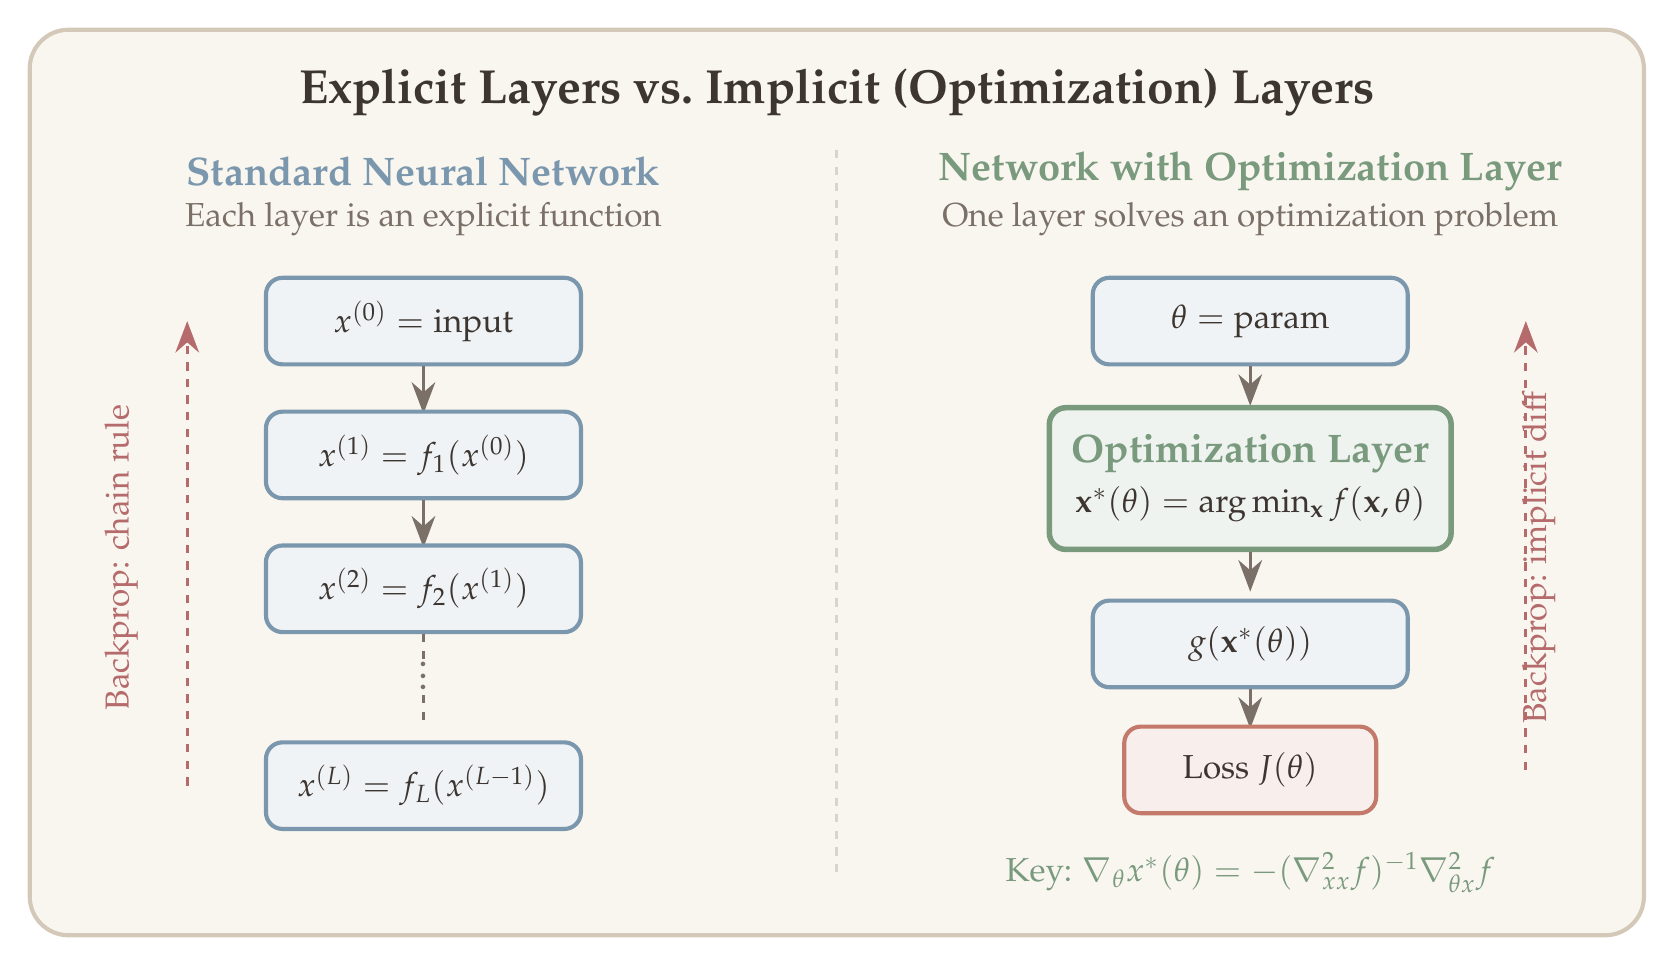
\begin{tikzpicture}[
  >={Stealth[length=4mm, width=3mm]},
  layer/.style={rounded corners=6pt, line width=1.5pt, minimum height=1.1cm,
                minimum width=4.0cm, align=center, text=dkbrown, font=\large, inner sep=8pt},
]

% Background
\fill[cream, rounded corners=14pt] (-0.5,-0.5) rectangle (20,11);
\draw[border, line width=1.5pt, rounded corners=14pt] (-0.5,-0.5) rectangle (20,11);

% Title
\node[font=\LARGE\bfseries, text=dkbrown] at (9.75,10.2) {Explicit Layers vs.\ Implicit (Optimization) Layers};

% ============ Left: Standard Neural Network ============
\node[font=\Large\bfseries, text=stblue] at (4.5,9.2) {Standard Neural Network};
\node[font=\large, text=wmgray] at (4.5,8.6) {Each layer is an explicit function};

% Layer chain
\node[layer, fill=stblue!12, draw=stblue] (l0) at (4.5,7.3) {$x^{(0)} = \text{input}$};
\draw[wmgray, line width=1.2pt, ->] (l0.south) -- ++(0,-0.6);

\node[layer, fill=stblue!12, draw=stblue] (l1) at (4.5,5.6) {$x^{(1)} = f_1(x^{(0)})$};
\draw[wmgray, line width=1.2pt, ->] (l1.south) -- ++(0,-0.6);

\node[layer, fill=stblue!12, draw=stblue] (l2) at (4.5,3.9) {$x^{(2)} = f_2(x^{(1)})$};
\draw[wmgray, line width=0.8pt, dashed] (l2.south) -- ++(0,-0.4);
\node[font=\Large, text=wmgray] at (4.5,2.9) {$\vdots$};
\draw[wmgray, line width=0.8pt, dashed] (4.5,2.55) -- ++(0,-0.4);

\node[layer, fill=stblue!12, draw=stblue] (lL) at (4.5,1.4) {$x^{(L)} = f_L(x^{(L-1)})$};

% Backward label arrow
\draw[rosefade, line width=1pt, dashed, ->] (1.5,1.4) -- (1.5,7.3);
\node[font=\large, text=rosefade, rotate=90, anchor=south] at (1.0,4.3) {Backprop: chain rule};

% ============ Divider ============
\draw[wmgray!30, line width=1pt, dashed] (9.75,0.3) -- (9.75,9.5);

% ============ Right: Network with Optimization Layer ============
\node[font=\Large\bfseries, text=sage] at (15,9.2) {Network with Optimization Layer};
\node[font=\large, text=wmgray] at (15,8.6) {One layer solves an optimization problem};

% Input
\node[layer, fill=stblue!12, draw=stblue] (r0) at (15,7.3) {$\theta = \text{param}$};
\draw[wmgray, line width=1.2pt, ->] (r0.south) -- ++(0,-0.5);

% Optimization layer (special)
\node[layer, fill=sage!12, draw=sage, line width=2pt, minimum height=1.8cm, minimum width=5.0cm] (opt) at (15,5.3) {%
  {\Large\bfseries\color{sage}Optimization Layer}\\[4pt]
  $\mathbf{x}^*(\theta) = \arg\min_{\mathbf{x}} f(\mathbf{x}, \theta)$
};
\draw[wmgray, line width=1.2pt, ->] (opt.south) -- ++(0,-0.5);

% Downstream NN
\node[layer, fill=stblue!12, draw=stblue] (rg) at (15,3.2) {$g(\mathbf{x}^*(\theta))$};
\draw[wmgray, line width=1.2pt, ->] (rg.south) -- ++(0,-0.5);

% Loss
\node[layer, fill=terracotta!12, draw=terracotta, minimum width=3.2cm] (loss) at (15,1.6) {Loss $J(\theta)$};

% Backward label arrow
\draw[rosefade, line width=1pt, dashed, ->] (18.5,1.6) -- (18.5,7.3);
\node[font=\large, text=rosefade, rotate=90, anchor=south] at (19.0,4.3) {Backprop: implicit diff};

% Key insight at bottom
\node[font=\large, text=sage] at (15,0.3) {Key: $\nabla_\theta x^*(\theta) = -(\nabla^2_{xx} f)^{-1} \nabla^2_{\theta x} f$};

\end{tikzpicture}
\end{document}
